\chapter{VPN}

Questo capitolo rappresenta la versione modificata dello studio che ho fatto
come primo passo della mia attività di tesi, in cui ho fatto una ricerca
sulle principali tecnologie di VPN esistenti, allo scopo di individuare
quali potessero soddisfare i requisiti di MoonCloud.\\
In particolar modo, il requisito più importante è la necessità di non dover
modificare la configurazione di rete nella rete target, soprattutto, non è
pensabile dover configurare delle rotte sul/sui router della rete target per
consentire la comunicazione tra tale rete e quella di MoonCloud.

\section{Introduzione}
\textit{VPN} è l'acronimo di \textit{Virtual Private Network}, ed indica diverse
tecnologie e protocolli utilizzati per, sostanzialmente, connettere tra loro
diversi reti locali geograficamente non contigue, oppure per connettere singoli host
ad una rete,
od anche singoli host tra loro. Questa \textit{connessione} avviene a diversi livelli dello stack
ISO/OSI, principalmente al livello 2 od al livello 3.\\
Si possono realizzare diverse topologie:
\begin{description}
  \item[Remote Access]Si realizza questa configurazione quando si vuole un connettere
  uno o più host ad una rete. Un esempio classico è quello di dipendenti che connettono
  il proprio dispositivo (PC, tablet, smartphone, etc \ldots) alla rete aziendale
  quando non si trovano in sede, potendo così accedere alle risorse che normalmente
  avrebbero disponibili solo se si trovassero fisicamente nella sede fisica dell'azienda.
  \item[LAN-to-LAN]A volte ci si riferisce a questa topologia anche come \textit{Intranet
  VPN}. In questo caso, si utilizza una VPN per connettere tra di loro due o più
  reti che sono geograficamente dislocate in posti diverse. E' molto utile per aziende
  che hanno più sedi sul territorio (anche in diversi stati), e che desiderano connettere
  tra di loro le reti di ciascuna sede.
  \item[Extranet VPN]Si tratta di un caso speciale di \textit{Intranet VPN}, e si realizza
  quando quando l'accesso ad una certa rete viene ristretto, ovvero è possibile accedere
  solo ad alcune sue parti mediante VPN.
\end{description}
Ma cosa significa davvero \textit{connettere tra di loro più reti}? La domanda sorge
spontanea, poiché una volta che due reti sono in Internet, in qualche modo
esse sono (indirettamente) connesse tra loro. In Internet, una normale rete privata
raggiunge solo le risorse che altre reti hanno rese disponbili su Internet,
siano esse dei server web o dei server mail.
Semplificando, si potrebbe dire che le varie reti accedono alle varie risorse delle
altre \textit{a livello di protocolli applicativi}.\\
Nel caso delle VPN, \textit{connettere tra di loro più reti a diversi livelli dello
stack ISO/OSI (o TCP/IP)} significa realizzare un collegamento \textit{ad un livello
più basso di quello applicativo}. La maggior parte delle VPN realizza un collegamento
al livello 2 od al 3, e questo ha i seguenti effetti pratici sulle $n$ reti connesse
tra di loro in VPN:
\begin{itemize}
  \item livello 2: le reti si trovano all'interno di un unico spazio di indirizzi IP
  (con stesso indirizzo di rete), ed è \textit{come se fossero separate da uno switch}.
  \item Livello 3: le diverse reti sono ciascune in uno spazio di indirizzamento separato,
  ed è \textit{come se fossero separate da un router}.
\end{itemize}
Supponendo che vi siano due reti, $A$ e $B$, connesse tramite una VPN al livello 3,
un host della rete $A$ può accedere a \textit{tutte} le risorse della rete $B$,
non solo quelle che $B$ espone verso la rete Internet.


Si distinguono tre tipologie di VPN:
\begin{description}
  \item[Secure VPN]Una VPN realizzata utilizzando crittografia dei dati in transito
  tra i diversi host/reti coinvolte, \textit{secure} poiché l'utilizzo di algoritmi
  crittografici (ammesso che siano utilizzati correttamente) garantiscono che nessun
  attaccante che intercetti tale traffico sia in grado di decifrarlo o alterarlo in
  qualsiasi modo.
  \item[Trusted VPN]Sono fornite dagli ISP, i quali garantiscono che nessun'altro
  cliente sia sullo stesso circuito VPN, \textit{trusted} poiché ci si fida di
  questa garanzia, inoltre, non vengono fornite particolari proprietà di sicurezza
  mediante protocolli crittografici.
  \item[Hybrid VPN]Termine che indica una VPN composta da tratti \textit{Secure}
  e da tratti \textit{Trusted}.
\end{description}
Di seguito, ci si concentrerà esclsuivamente sulla prima tipologia, poiché essa è
quella di interesse per MoonCloud.


\section{Anatomia}
Nell'ambito delle VPN del primo tipo, un pricipio base su cui si fonda il loro
funzionamento è quello dell'\textit{incapsulamento}. Si tratta di un termine
ben noto nell'ambito dei protocolli di rete, che può essere sintetizzato come
di seguito. Siano $A, B$ due protocolli di rete, con $A$ che si trova ad un livello
più basso rispetto ad $B$ (quindi più vicino al \textit{fondo} della pila
protocollare). Entrambi i protocolli hanno un \textit{header} ed un
\textit{payload}.\\
Si dice che \textit{B incapsula A} quando il payload di $B$ è costituito dall'intero
pacchetto di $A$, come mostrato in figura \ref{fig:encaps}.
E' importante notare che l'incapsulamento può essere ulteriormente generalizzato,
non è richiesto che $A$ sia di un livello più basso rispetto a $B$. Nello pila
di protocolli di rete, sia essa ISO/OSI o TCP/IP, l'incapsulamento è il modo di
procedere normale, per cui ad esempio un segmento TCP ha nel proprio payload
un intero pacchetto IP, il cui a sua volta ha come payload un intero frame Ethernet.


Di seguito si procede a dare una descrizione del funzionamento della maggior parte
delle VPN secure, iniziando con il definire con \textit{protocollo VPN}
il procollo utilizzato nel collegamento tra le reti/host.
Generalmente si distingue tra VPN client e VPN server, sebbene
una volta stabilito il collegamento, il protocollo VPN sia spesso peer-to-peer (un
pò come nel protocollo TLS, nella fase di \textit{handshake} vi è una chiara distinzione
tra client e server, ma una volta stabilita una connessione le due parti sono di fatto
paritetiche); in ogni caso vi è sempre un host che inizia la connessione.\\
Il VPN server può ricevere più connessioni dai VPN client, i quali in quanto tali
iniziano la connessione verso il server. A seconda della topologia/tecnologia,
i client possono essere responsabili di connettere alla rete del server la rete
a cui essi appartengono; viceversa, il server \textit{può} rendere visibile ai client
la rete cui appartiene. Altrettanto opzionalmente,
il server può connettere tra di loro i diversi client e le loro reti (nel senso che
i client possono comunicare tra loro anziché solo con il server/con la rete del server).\\
Per poter effettivamente collegare tra loro più \textit{reti}, il VPN \textit{peer}
deve avere i seguenti \textit{punti di contatto}:
\begin{itemize}
  \item collegamento con l'altro peer, raggiungibile tramite la rete Internet;
  \item punto di ricezione da cui riceve pacchetti provenienti dagli host della
  rete in cui esso si trova e diretti alla rete dell'altro peer;
  \item punto di invio al quale l'host invia i pacchetti provenienti dalla rete dietro
  la VPN
  e diretti ad host della propria.
\end{itemize}
Il collegamento di cui al primo punto si realizza spesso (ma non sempre) con un socket,
mentre gli ultimi due punti si realizzano con una \textit{scheda di rete virtuale}.\\
Nel collegamento lungo il socket, la tecnologia VPN definisce un protocollo (che ovviamente
garantisca proprità di sicurezza), può essere un protocollo già esistente come TLS,
oppure uno sviluppato ad hoc.\\
Una scheda di rete virtuale (o virtual NIC -- Network Interface Card) è una
scheda di rete che esiste nel kernel del sistema
operativo ma che non ha un corrispettivo fisico. Se ne può creare una al livello 2
od al livello 3 (utilizzando \texttt{TUN}, modulo del
kernel implementato in diversi sistemi operativi). Una scheda di rete
al livello 3 è dotata di un indirizzo IP proprio come ogni NIC reale.\\
Una scheda di rete virtuale è associata ad un software che compie operazioni su essa,
e, come per ogni scheda di rete, tali operazioni sono quelle di invio e ricezione.
\begin{description}
  \item[Inviare]Il software associato invia
  o funzione equivalente) un pacchetto sulla NIC, l'effetto è che tale
  pacchetto viene \textit{ricevuto} dal kernel del sistema operativo e processato
  come un qualsiasi altro pacchetto, pertanto l'OS deciderà
  dove e come inviarlo, e se applicare ulteriori trasformazioni.
  \item[Ricevere]Il sistema operativo riceve un pacchetto che ha per indirizzo destinazione
  quello delle scheda di rete virtuale, l'OS quindi inoltra il pacchetto alla NIC
  virtuale in questione, l'effetto è che il software associato riceve i dati
  che il sistema operativo ha inoltrato. Il pacchetto che viene inoltrato alla NIC
  può essere benissimo un pacchetto inviato da un altro host, e che quindi è arrivato
  al sistema operativo mediante una scheda di rete reale (oppure un'altra virtuale).
\end{description}
A livello di processo associato alla NIC, \textit{inviare un dato alla NIC} significa
chiamare la funzione \texttt{write()}, mentre \textit{ricevere} significa
utilizzare \texttt{read()} (o funzioni equivalenti).


L'idea di base è che ciò che il software VPN legge dalla scheda di rete virtuale
è ciò che è destinato ad un altro membro della VPN, e quindi venga incapsulato secondo
il protocollo VPN usato. Allo stesso modo, ciò che si riceve dal socket è destinato
alla proprio rete (salvo il caso si tratti di un server che connette più client), pertanto
viene scritto sulla NIC, per essere dato in gestione al proprio sistema operativo in
modo che possa inoltrarlo al destinatario.\\
Due note fondamentali che occorre sempre tenere presenti:
\begin{itemize}
  \item se si realizza una VPN al livello 3, tutte le reti partecipanti devono
  avere degli spazi di indirizzamento diversi.
  \item In una VPN al livello 2, tutte le reti partecipanti devono stare
  nella stessa rete IP.
\end{itemize}


Per capire meglio quanto spiegato, si procede con un esempio.
Si supponga ora di voler configurare una certa \textit{VPN X}, e che si voglia realizzare una
topologia LAN-to-LAN tra due rete $A, B$, in cui nella prima si trova il server VPN $X$,
nella seconda naturalmente si trova il client.  Lo scenario è il seguente:
\begin{itemize}
  \item rete $A$: indirizzo di rete: \texttt{192.168.1.0/24}
  \item rete $B$: indirizzo di rete: \texttt{192.168.10.0/24}
  \item indirizzo interno del server VPN in $A$: \texttt{192.168.1.200}
  \item indirizzo pubblico del server VPN: \texttt{2.7.200.70}
  \item indirizzo interno del client VPN: \texttt{192.168.10.20}
\end{itemize}
Per brevità, ci si riferirà al server con $s$, ed al client con $c$. Si definiscono
infine gli host \texttt{192.168.1.5} come $a_5$, e \texttt{192.168.10.5} in $b_5$, ed infine
si suppone che gli indirizzi IP
dei default gateway delle due reti finiscano in \texttt{.254}.\\
Per il momento non ci si concentra troppo sulla configurazione delle rotte, supponendo che i
pacchetti arrivino
agli host corretti. Si anticipa soltanto che in tutte le reti partecipanti alla VPN
(in questo caso $A$ e $B$), occorre configurare \textit{almeno una rotta}; nel capitolo in cui si descrivono le configurazioni di OpenVPN,
questo aspetto viene affrontato nel dettaglio.\\
Si vede quindi cosa succede quando $b_1$ vuole comunicare con $a_1$, posto che il
collegamento VPN tra $c$ ed $s$ sia già stato stabilito con successo. Si precisa che
si utilizza il termine generico \textit{pacchetto} per indicare un qualsiasi messaggio
di un qualsiasi protocollo di rete.
\begin{itemize}
  \item Il pacchetto da $b_1$ viene inviato, e quindi ricevuto da $c$.
  \item Il sistema operativo di $c$ invia il pacchetto alla scheda di rete virtuale
  della VPN.
  \item Il pacchetto originale viene incapsulato da $c$ in un nuovo pacchetto secondo
  il protocollo VPN, quindi inviato ad $s$ e da $s$ ricevuto.
  \item $s$ decifra (ed effettua verifiche di autenticità, integrità, ecc\ldots) il
  pacchetto, a questo punto il risultato della decifratura è un pacchetto esattamente
  uguale a quello generato al punto 1.
  \item $s$ scrive il pacchetto sulla propria scheda di rete virtuale.
  \item L'OS di $s$ riceve il pacchetto, lo invia a $a_1$.
\end{itemize}


Il protocollo di trasporto preferito è UDP in quanto introduce meno overhead rispetto al TCP. A causa
dei particolari requisiti di MoonCloud, ci si è concentrati invece su soluzioni che
supportassero il TCP, questo perché è possibile che nelle reti target UDP sia bloccato,
mentre è infattibili ritenere che TCP stesso sia bloccato. Probabilmente vi saranno
delle restrizioni, e nel caso in cui proprio la VPN non riesca a funzionare si può sempre
chiedere di aprire una porta sul firewall, l'importante è non essere troppo invasivi.


\section{Topologie}
In questa sezione si esaminano le diverse topologie realizzabili per connettere una rete
target a MoonCloud. Non tutte le tecnologie consentono di realizzare le topologie qui
dettagliate.
\begin{description}
  \item[\textit{LS - Local Server}]In questa configurazione si prevede di installare i
  VPN server in MoonCloud, mentre nelle reti target si porta (o si installa) il device
  VPN client, il quale è incaricato di connettersi al VPN server. Un server può essere
  potenzialmente responsabile per più reti client diverse. I container che fanno analisi
  (o l'host su cui sono in esecuzione)
  sono configurati per inoltrare i pacchetti al VPN server, il quale li invia alla rete
  target mediante il collegamento VPN.
  \item[\textit{RSMC - Remote Server Multi Client}]Opposta alla precedente, in \textit{RSMC}
  si installa un singolo VPN server nelle reti target. In una configurazione di tipo
  \textit{Multi Client}, ciascun Docker host è connesso direttamente in VPN con il server, il
  quale, una volta ricevuti i pacchetti dalla VPN li invia agli host target.
  \item[\textit{RSSC - Remote Server Single Client}]Simile ad \textit{RSMC}, il VPN
  server è presente nella rete target, tuttava in MoonCloud si realizza, per ciascuna rete
  target, un unico VPN client, a cui i Docker host responsabili per una certa rete target inviano
  i pacchetti per tale rete. Il client invia quindi in pacchetti lungo la VPN al server,
  che quindi provvede ad inoltrarli agli host nella rete target.
\end{description}
Nelle configurazioni di tipo \textit{Remote Server}, è necessario che il server sia
direttamente raggiungibile da MoonCloud, e quindi deve disporre di un indirizzo IP pubblico.
Si è supposto ragionevolmente che la rete target disponga di un collegamento ad Internet, e che
sia dietro router/firewall che esegua NAT. Come tale, la rete target è raggiungibile
mediante un indirizzo IP pubblico dinamico. Poiché vi è NAT, è fondamentale che il server disponga
di un qualche meccanismo di NAT Traversal, poiché si vuole evitare di dover configurare
port forwarding sul router del cliente.\\
Vi sono naturalmente casi in cui non c'è NAT, ma sono una minoranza.


Già in questa fase iniziale di studio avevo previsto l'utilizzo del \textit{NAT al contrario},
un termine coniato qui per indicare un particolare utilizzo del NAT. Si supponga di
essere nella situazione delle due reti elencate precedentemente, ma in cui non vi sia
possibilità di intervenire sulle rotte nella rete $A$ (non si sono ancora viste quali rotte,
ma si è detto che sono necessarie delle rotte introdotte sull'intera rete) perché essa è
la rete target, e quindi si vogliono limitare gli interventi in essa.
I pacchetti inoltrati da $s$ (nella rete $A$) verso la rete e provenienti da $B$, hanno
come indirizzo IP sorgente un indirizzo IP in $B$. Una volta che tali pacchetti
sono stati ricevuti da un host di $A$, esso non ha modo di sapere che le risposte devono
tornare ad $s$ (proprio perché non vi sono rotte configurate), e quindi invierebbe il
pacchetto al proprio default gateway, che quindi lo dropperebbe (trattandosi di una
destinazione con indirizzo IP privato).\\
Il \textit{NAT al contrario} consiste nell'applicare NAT sui pacchetti
da $s$ (o da $c$ a seconda se sia client o server nella rete target) provenienti dalla
VPN e destinati alla propria rete: in questo modo raggiungono l'host target con l'indirizzo IP
di $s$, che si trova nella stessa rete del target, e per tale ragione il target può
inviare ad $s$ le risposte senza passare dal default gateway.\\
Questo meccanismo è stato descritto in maniere molto sintetica, poiché è una soluzione che è stata
davvero applicata, viene analizzato molto più nel dettaglio nel capitolo dedicato alle configurazioni
di OpenVPN.\\
Tra queste topologie, si anticipa che quella scelta è \textit{LS}.


\section{Motivazioni}
TODO.

\section{Introduzione alle tecnologie}
La tabella \ref{tbl:vpn-comparison} riassume le principali tecnologie VPN. Nella
penultima colonna, con \textit{firewall stringenti} ci si riferisce a firewall che
lavorano a livello applicativo.
\begin{table}\label{tbl:vpn-comparison}
  \begin{tabular}{|p{3.3cm}|p{2.7cm}|p{3.1cm}|p{1.7cm}|p{3cm}|}
    \hline
    Technology & Procollo di trasporto & Protocollo incapsulato & Passa fw. stringenti & NAT Traversal\\
    \hline
    OpenVPN & TCP/UDP & Ethernet/IP & No & Sì, keepalive-based\\
    \hline
    IPsec (IKEv2) & IPsec & IP & No & Sì\\
    \hline
    SoftEther & HTTPS (anche ICMP, DNS) & Ethernet/IP & Sì & Sì, parzialmeente\\
    \hline
    L2TP/IPsec (IKEv1) & IPsec & IP & No & Sì (con SoftEther)\\
    \hline
    \hline
    SSTP & HTTPS & PPP (IP) & Sì & Sì (con SoftEther)\\
    \hline
    OpenConnect (Cisco Any Connect)& DTLS e HTTPS & IP & Sì con HTTPS & ?\\
    \hline
    OpenSSH & SSH & Ethernet/IP/TCP & No & ?\\
    \hline
    WireGuard & WireGuard & IP & No & Sì, keepalive-based \\
    \hline
    L2TPv3/IPsec & IPsec & Ethernet (e altri layer 2) & No & Sì (con IKEv2 o SoftEther)\\
    \hline
    EtherIP/IPsec & IPsec & Ethernet & No & Sì (con IKEv2 o SoftEther)\\
    \hline
    PPTP & GRE & PPP (IP and others) & No & No\\
    \hline
  \end{tabular}
  \caption[Tecnolgie per VPN]{Principali tecnologie per VPN.}
\end{table}

Prima di proseguire, occorre subito chiarire che il problema principale dell'usare una VPN
è che \textbf{spesso è necessario configurare almeno un firewall} o default gateway o router di
confine. Per questo motivo
si cercherà, nei limiti del possibile, di valutare quali opzioni sono più \textit{soft}
da questo punto di vista.\\
Con le VPN si possono realizzare due topologie:
\begin{itemize}
  \item \textbf{Remote Access}: in questa configurazione si connette un host ad una LAN.
  Sulla LAN sarà necessario installare il componente server, sul PC il componente client
  dell'infrastruttura VPN\footnote{Nella maggior parte delle tecnologie VPN vi è una distinzione
  tra client e server, anche nei casi \textit{peer-to-peer} come IPsec.}.
  \item \textbf{LAN-to-LAN}: si realizza una connessione tra due reti locali, in modo che gli
  host di ciascuna rete possano connettersi agli host dell'altra, e viceversa (a livello 2
  o a livello 3). Per fare ciò, su un host della rete si installa il server, su un host
  dell'altra il client oppure un altro componente specifico. Attuando le opportune configurazioni, i due host sono responsabili
  di instradare tutto il traffico della propria rete verso l'altro. Il problema, come si vedrà
  più avanti, è che per far sì che tutto funzioni occorre aggiungere delle rotte in entrambe le
  reti.
\end{itemize}
Esiste anche \textbf{extranet}, che corrisponde a Remote Access o LAN-to-LAN con accesso ristretto alle
risorse della rete remota. Visto lo scopo di questo documento, non ci si sofferma su questa differenza.
Da ora in poi si userà il termine \textit{rete target} per indicare la rete che MoonCloud analizza.\\
Le due topologie si traducono nel seguente modo per l'architettuta MoonCloud:
\begin{itemize}
  \item Remote Access: in questo caso i container diventano client del server VPN installato nella rete
  target\footnote{Si tenga presente che è
  possibile \textit{invertire} questo paradigma, ed avere il server in MoonCloud.}.
  \item LAN-to-LAN: i container che fanno analisi e la rete target sono connessi in un'unica rete.
  Sono possibili soluzioni per cui il server si installa su MoonCloud oppure nella rete target.
\end{itemize}
Ciascuna di queste due strade ha vantaggi e svantaggi, che verranno dettagliate tecnologia per tecnologia.\\
Ora si passa a valutare le singole tecnologie VPN. Per ciascuna di esse si fornisce una overview
generale, si elencano i passi necessari per raggiungere una certa configurazione
(in modo da avere un'idea della complessità), si valutano le diverse topolgie posssibili. Si conclude
infine suggerendo quali sono le opzioni migliori.


Un'ultima nota di proseguire: durante tutto questo capitolo ed il prossimo, si utilizzerà
il termine \textit{pacchetto} per indicare una generica sequenza di byte di un generico
protocollo, presente in un certo momento in un host dopo essere stata ricevuta o prima
di essere inviata, oppure in viaggio sulla rete. Sono perfettamente consapevole che per
ogni livello dello stack ISO/OSI vi sia un termine specifico per indicare tale
sequenza, ad esempio \textit{frame} per il livello 2 con Ethernet, oppure \textit{datagrammi}
per il protocollo UDP, e così via. Tuttavia, come si è visto dalla tabella \ref{tbl:vpn-comparison},
le VPN possono funzionare su diversi protocolli di trasporto (non solo al livello 4),
e possono altresì incapsulare
pacchetti di livelli divrersi. Per questa ragione ho scelto di utilizzare
\textit{indiscriminatamente} il termine \textit{pacchetto} per riferirmi ad essi.


% TODO check if I already said this
Tra le soluzioni indicate di seguito, la prima scelta è stata SoftEther. Per motivi che
verranno spiegati in seguito, la soluzione definitiva è poi OpenVPN.

\section{OpenVPN}
\subsection{Overview}
OpenVPN è un software open source molto diffuso per la creazione di VPN,
è in grado di incapsulare pacchetti al livello 2 o 3, e come protocollo di trasporto
può usare TCP o UDP. E' la soluzione che è stata scelta, ed in questo capitolo
se ne presenta una panoramica, mentre viene approfondita nel dettaglio
nel prossimo.


Per ciascun tunnel VPN, vengono create due connessioni separate:
\begin{itemize}
  \item \texttt{Control Channel} cifrato con TLS per scambiarsi informazioni di servizio
  \item \texttt{Data Channel} cifrato con un protocollo simile  a TLS per lo scambio
  di dati.
\end{itemize}
Entrambe le connessioni sono multiplexate su di un unico protocollo di trasporto
da OpenVPN, sia esso TCP o UDP.
OpenVPN è una tecnologia ampiamente usata per creare VPN.
La figura \ref{fig:openvpn-sec} mostra un semplice schema del suo funzionamento.\\
\begin{figure}[h!]
  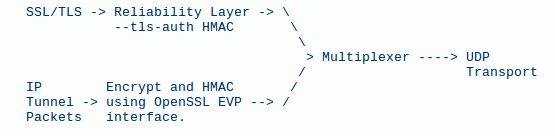
\includegraphics[scale=0.4]{img/openvpn_sec}
  \caption[Il multiplexing di OpenVPN]{Il multiplexing di OpenVPN: si vede come
  le due connessioni siano multiplexate su un unico protocollo L4, in questo caso UDP.}
  \label{fig:openvpn-sec}
\end{figure}
OpenVPN viene distribuitpo anche in una versione \textit{enterprise} a pagamento: si chiama
\textit{OpenVPN AS -- Access Server}, offre una web GUI, sicuramente più intuitiva
rispetto ai file di configurazione con cui si amministra la versione open source
(detta \textit{Community Edition}). D'ora in poi ci si concentra su quest'ultima
versione, a livello di VPN le funzionalità sono le stesse; per una comparazione tra
le due versioni si veda
\cite{openvpn-comparison}.\\
L'infrastruttura OpenVPN si compone di:
\begin{itemize}
  \item server: in grado di connettere tra loro diversi client, è possibile regolare
  il fatto che diversi client possano \textit{vedersi} tra loro o meno
  \item client, il quale si connette al server.
\end{itemize}
E' necessario che il server abbia un indirizzo IP pubblico, oppure dinamico e raggiungibile con un DNS. E' possibile
usare servizi che dinamicamente seguono gli aggiornamenti agli indirizzi IP, in modo che i client usino
sempre un unico nome per raggiungerlo. Si noti che questa tecnologia (\textit{dynamic DNS}) è integrata in SoftEther.\\
E' possibile avere il server dietro un firewall, a patto di abilitare il port forwarding dal gateway al server.\\
L'autenticazione tra i diversi membri della VPN può essere fatta in due modi:
\begin{itemize}
  \item certificate-based, cioè autenticazione basata su chiavi pubbliche e certificati
  X509. I passi da seguire sono:
  \begin{itemize}
    \item creazione di una nuova CA, quindi della coppia di chiavi e di un certificato
    self-signed
    \item ciascun membro della VPN deve avere la propria coppia di chiavi e certificato
    \item il certificato della CA deve essere presente in ogni macchina partecipante
  \end{itemize}
  \item PSK: si generano a priori delle chiavi statiche, che devono essere distribuite
  su ciascun host membro della VPN. Questa modalità non è consigliata, in quanto
  se un host venisse in qualche modo compromesso, occorrerebbe cambiare tutte le chiavi.
  Inoltre non si garantisce \textit{perfect forward secrecy}: se un avversario
  intercettasse il traffico sull VPN e poi ottenesse queste chiavi potrebbe
  decifrarlo senza problemi.
\end{itemize}
E' possibile inoltre configurare anche username e password per ciascun client.

Si possono realizzare sia topologie \textit{Remote Access} sia \textit{LAN-to-LAN},
per ciò che concerne la configurazione effettiva di OpenVPN, le due cose
sono praticamente identiche, se si vuole realizzare l'ultima topologia occorre
però definire diverse rotte nelle reti partecipanti. In particolare,
l'host VPN (client o server) deve essere configurato come gateway per le reti
raggiungibili mediante l'\textit{altro} host VPN a cui è connesso.

Per ciò che concerne la versione free di OpenVPN, client e server sono implementati
nello stesso singolo programma.

\subsection{OpenVPN e MoonCloud}
Si passa ora ad analizzare le possibilità di implementare OpenVPN in MoonCloud al livello 3. Il primo step
da fare è decidere dove posizionare il server: nel cloud o nella rete target?
\begin{description}
  \item[\textbf{Nel cloud}]Con questa opzione si preparano nella rete MoonCloud una serie
  di VM destinate ad essere VPN server; se esse sono configurate propriamente, ciascun server
  può servire diverse reti target. I probes
  hanno delle rotte configurate del tipo \texttt{rete target via VPN server}.
  Nelle reti dei client si porta quindi una appliance che quindi client di un server in MoonCloud.
  Tale appliance deve rendere visibile l'intera rete (possibilmente anche più di una) nella VPN. In
  particolare si pone un problema di routing nella rete target a prescindere che lì vi sia
  il server od il client, pertanto è descritto tra qualche riga.
  \item[\textbf{Nella rete target}]Portare un server nella rete target subito un problema: deve
  essere raggiungibile dall'esterno, e questo non è per niente facile poiché la maggior parte
  delle reti target utilizzano NAT, e quindi gli host interni non sono direttamente raggiungibili
  dall'esterno, se non con port forwarding sul router. Chiedere ai clienti di configurare
  questo non è pensabile, pertanto questa opzione non è stata consigliata ed infatti
  non è stata presa effettivamente in considerazione come soluzione praticabile.
  In via del tutto ipotetica, se si fosse scelta questa strada si sarebbe poi
  dovuto decidere anche come effettivamente configurare i client VPN. Ad esempio,
  sarebbe stato possibile connettere direttamente al server ciascun Docker host, oppure
  dedicare un host al compito apposito di servire i vari Docker host nel collegamente VPN.
\end{description}
Il problema comune ad entrambe queste due opzioni è il seguente: in una configurazione
\textit{normale} i pacchetti provenienti dai probes e diretti ai target, una volta che
sono decifrati ed immessi nella rete dal VPN client (poiché l'opzione server
è stata scartata) hanno come indirizzo IP sorgente un IP che si trova nella rete MoonCloud,
ed i target non hanno modo di sapere che le risposte a tali pacchetti devono passare
per il VPN client. La soluzione a cui avevo già pensato in questa prima fase di studio
è stata quella del \textit{NAT al contrario}, per cui i pacchetti immessi nella rete
target dal VPN client vengono NAT-tati ed hanno come IP sorgente quello del VPN
client, che si trova nella stessa rete dei target e quindi le risposte torneranno
ad esso direttamente.

Senza NAT l'unica strada sarebbe stata configurare delle rotte sul default gateway
della rete target o su tutti gli host. In ogni caso, questa assieme a tutte
le altre soluzioni adottate per la VPN sono descritte molto dettagliatamente
nel prossimo capitolo.

% \begin{figure}
%   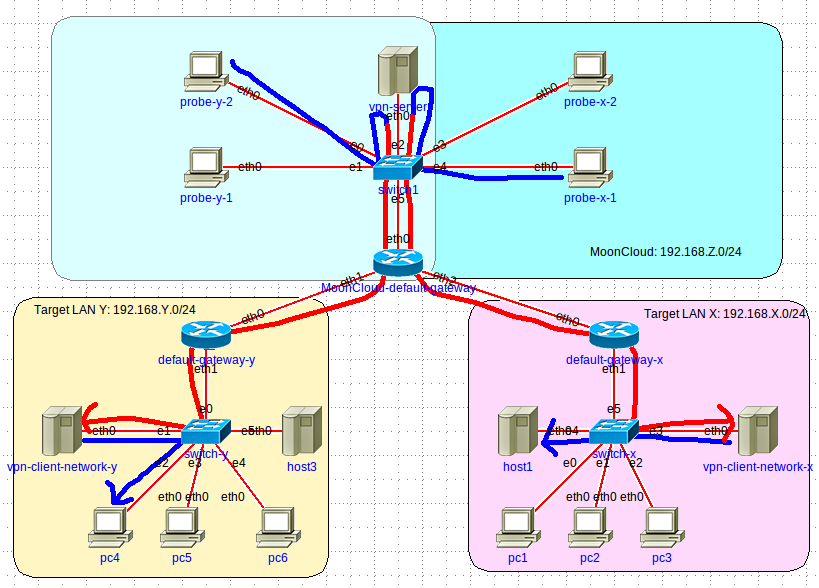
\includegraphics[scale=0.35]{img/sls}
%   \caption[Configurazione \textit{SLS (Single Local Server)}]{Configurazione \textit{SLS (Single Local Server)},
%   il server è in grado di collegare subnet con indirizzi IP diversi, a patto che tutto
%   sia configurato opportunamente. Le frecce rosse indicano il collegamento VPN, le frecce blu il traffico prima di essere inviato
%   e dopo essere stato decifrato dalla VPN.}
% \end{figure}

% \begin{figure}
%   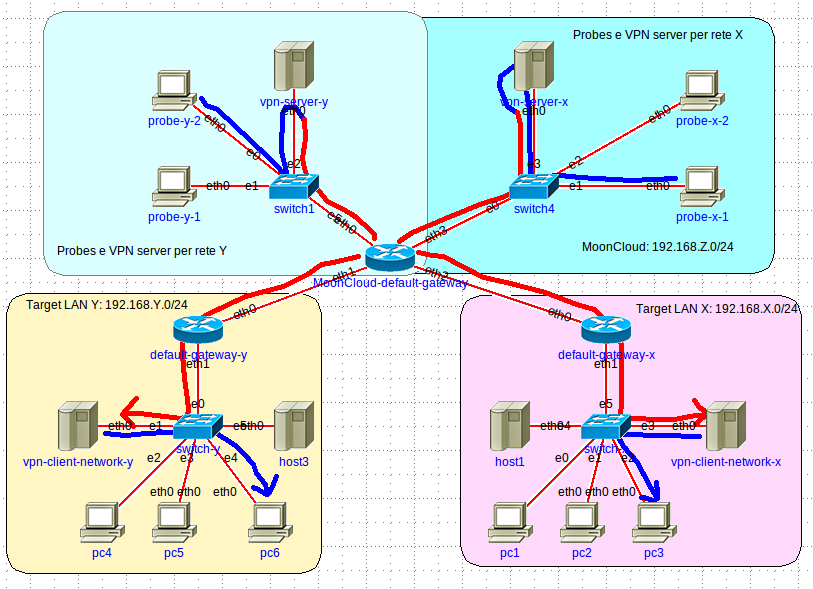
\includegraphics[scale=0.4]{img/mls}
%   \caption[Configurazione \textit{MLS (Multi Local Server)}]{Configurazione \textit{MLS (Multi Local Server)},
%   per ciascuna rete target si configura un VPN server che instrada il traffico dei containter (in blu) sulla VPN (in rosso).}
% \end{figure}

% \begin{figure}
% %   \centering
% %   \begin{minipage}[t]{0.5\textwidth}
%   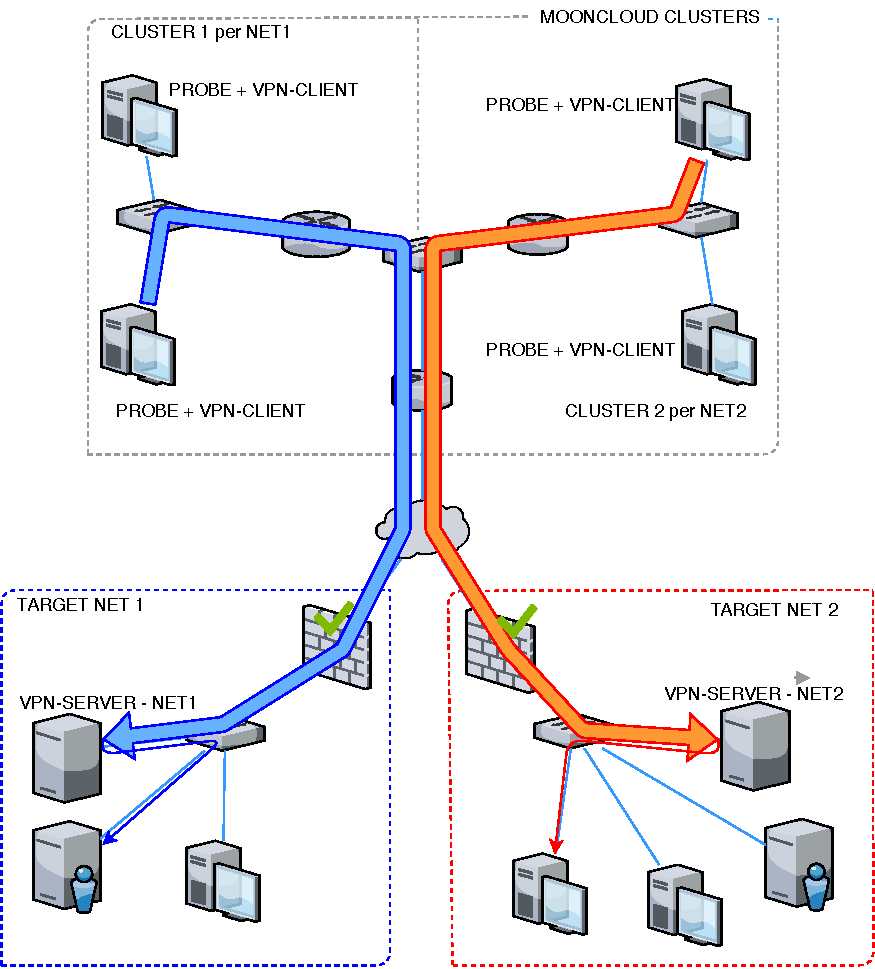
\includegraphics[scale=0.45]{img/rsmc}
%   \caption[Configurazione \textit{RSMC (Remote Server Multi Client)}]{Configurazione \textit{RSMC (Remote Server Multi Client)}.}
% \end{figure}
%   % \end{minipage}
%   % \hfill
%   % \begin{minipage}[t]{0.45\textwidth}
% \begin{figure}
%   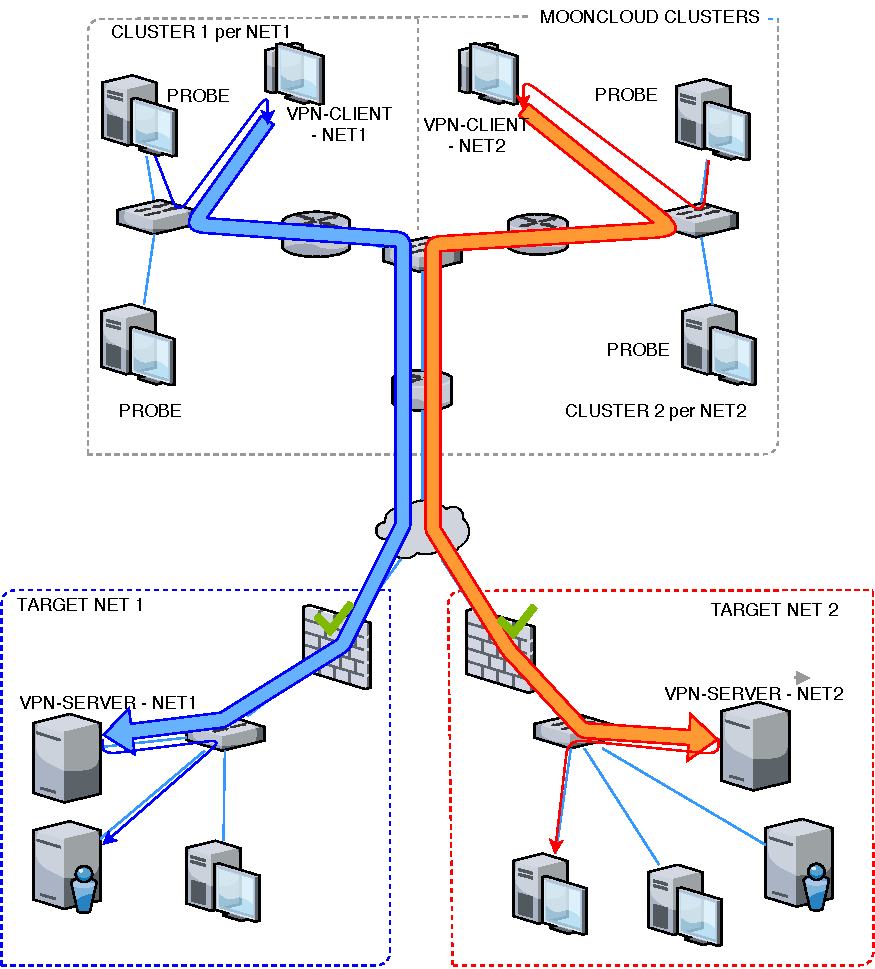
\includegraphics[scale=0.45]{img/rssc}
%   \caption[Configurazione \textit{RSSC (Remote Server Single Client)}]{Configurazione \textit{RSSC (Remote Server Single Client)}.}
%   % \end{minipage}
% \end{figure}

\subsection{Conclusioni}
Per ciò che concerne OpenVPN, si è consigliato di realizzare una soluzione \textbf{\textit{Local Server}} per
evitare di dover configurare port forwarding nella rete target. Nel caso in cui questo
problema non si dovesse presentare, ad esempio perché la rete target dispone di un
pool di IP pubblici, sarebbe possibile tentare la strada di un \textit{Remote Server}.
A causa di un mio errore, nella prima fase di studio avevo suggerito quest'ultima configurazione.

\section{SoftEther}
\subsection{Overview}
\texttt{SoftEther} \cite{softether} è una tecnologia per VPN molto particolare, sviluppata dallo studente
giapponese D. Nobori per la sua tesi di laurea magistrale,
è un progetto
attivamente sviluppato, open source e gratuito.\\
E' disponibile cross-platform, Linux, MAC OS X e Windows. Per
le versioni MAC OS X e Windows è disponibile un'interfaccia grafica sia per client
sia per server, che consente di fare configurazioni in maniera molto intuitiva; su Linux
bisogna cavarsela con file di configurazione ed una shell (\texttt{vpncmd}).


La particolarità di questo software è che in grado di gestire anche \textit{altri}
protocolli VPN, oltre ad uno sviluppato ad hoc:
\begin{itemize}
  \item SoftEther (VPN over HTTPS)
  \item OpenVPN (L2  e L3)
  \item SSTP (PPTP over TLS)
  \item L2TP/IPsec
  \item L2TPv3/IPsec
  \item EtherIP
\end{itemize}
Il grande vantaggio che dà l'utilizzo del protocollo SoftEther è l'incapsulamento in
HTTPS, per cui si usa tutta la sicurezza derivante da TLS, unitamente al fatto che
praticamente qualsiasi firewall lascerà passare tale traffico.\\
La figura \ref{fig:softether-archi} mostra come funziona SoftEther.


SoftEther è composto da diversi software:
% \begin{figuare}
%   \includegraphics{img/sofether_scheme}
%   \caption{}
% \end{figuare}
\begin{itemize}
  \item \textit{VPN Server}: il componente server in grado di gestire i multipli
  protocolli VPN
  \item \textit{Virtual Hub} che, a dispetto del nome, è uno switch che viene usato internamente
  dal VPN Server per collegare i diversi tunnel (uno per ogni protocollo)
  \item \textit{Virtual L3 Switch}: anche in questo caso il nome trae in inganno, poiché si tratta di un
  router che si utilizza in topologie LAN-to-LAN.
  \item \textit{Local Bridge}: componente del server che viene usato per collegare la rete dei Virtual Hub
  alla rete fisica su cui si trova il server VPN. E' necessario avere un'interfaccia di rete
  reale dedicata che sia connessa alla rete fisica (su cui non sia attivo nessun protocollo di rete);
  è possibile anche utilizzare una scheda di rete virtuale usando \texttt{TAP} al layer
  2\footnote{\texttt{TAP} è un modulo del kernel Linux che consente di creare NIC virtuali al livello 2.}.
  E' consigliabile
  una NIC di buona qualità, che possa lavorare in modalità promiscua. Non è obbligatorio
  avere questa seconda interfaccia, sebbene sia caldamente consigliato.
  \item \textit{VPN Bridge} è la combinazione di \textit{Virtual Hub} e \textit{Local Bridge} che consente
  di collegare tra loro diverse \textit{reti} in VPN (e non singoli host). E' utilizzato
  lato client per realizzare topologie LAN-to-LAN.
  \item \textit{VPN Client} è il classico componente client che connette un PC ad una VPN. Utilizza il
  protocollo SoftEther VPN sopra descritto. Come client si può comunque utilizzare un qualsiasi software che
  usi uno dei protocolli sopra citati. E' da utilizzare solo in configurazioni Remote Access.
\end{itemize}


\begin{figure}
  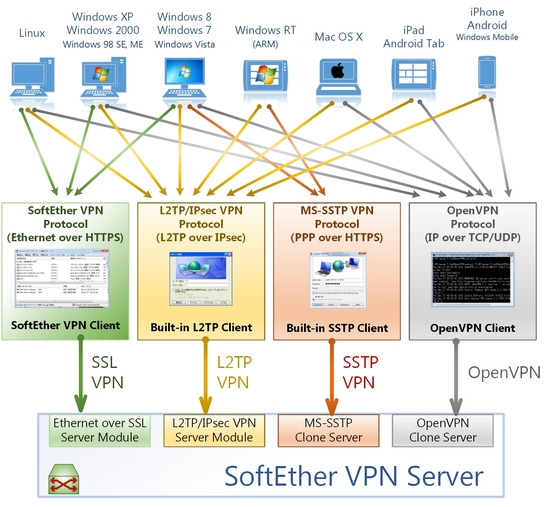
\includegraphics[scale=0.45]{img/softether_scheme}
  \caption[Il design di SoftEther]{Il design di SoftEther. Mediante il \textit{Virtual Hub} si \textit{collegano} i diversi
  moduli. \url{https://www.softether.org/@api/deki/files/4/=1.2.jpg?size=webview}}
  \label{fig:softether-archi}
\end{figure}
Con SoftEther si possono realizzare diverse topologie:
\begin{itemize}
  \item \textbf{Remote Access}. Si crea in maniera molto semplice una nuovo server, mediante la GUI o
  la linea di comando. Dal punto di vista logico si fanno i seguenti passaggi:
  \begin{enumerate}
    \item creazione di un nuovo server;
    \item creazione di un nuovo \textit{Virtual Hub} che ``riceve le connessioni'';
    \item connessione del \textit{Virtual Hub} alla scheda di rete del server (possibilmente dedicata a fare
    questo). Così facendo si dà accesso alla rete in cui si trova il server.
    \item Connessione al server utilizzando il software client.
    \begin{figure}
      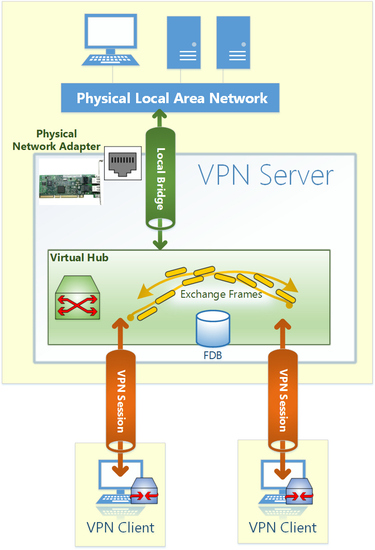
\includegraphics[scale=0.4]{img/softether_ras}
      \caption[Configurazione di SoftEther per Remote Access VPN]{
        Configurazione di SoftEther per Remote Access VPN.
        \url{https://www.softether.org/@api/deki/files/626/=1_remote2.jpg?size=webview}}
        \label{fig:softether_ras}
    \end{figure}
  \end{enumerate}
  \item \textbf{LAN-to-LAN}. E' possibile scegliere se collegare le diverse LAN
  a livello 2 o a livello 3.
  Una volta scelta la topologia che si preferisce si crea un \textit{VPN server}, poi occorre
  differenziare in base al livello.
  \begin{itemize}
    \item L2 \cite{softether-l2-lan-to-lan}:
    \begin{enumerate}
      \item sulla rete da connettere al server si crea un nuovo \textit{VPN Bridge}
      \item si connette il bridge al server (si chiama \textit{cascaded connection})
      \item si connette il bridge alla LAN locale utilizzando \textit{Local Bridge}.
      \begin{figure}
        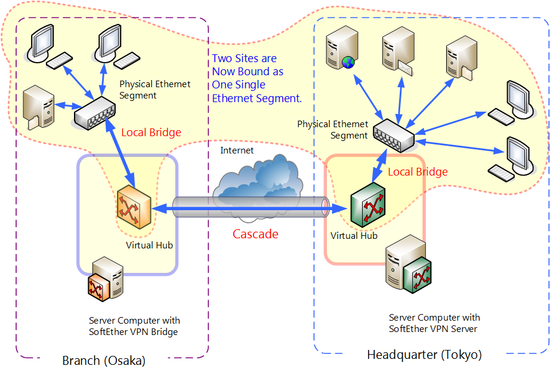
\includegraphics[scale=0.55]{img/softether_l2_lan_to_lan}
        \caption[Configurazione LAN-to-LAN con SoftEther al layer 2]{
          Configurazione LAN-to-LAN con SoftEther al layer 2.
          \url{https://www.softether.org/@api/deki/files/325/=10-5-1.png?size=webview}}
          \label{fig:softether_l2_lan_to_lan}
      \end{figure}
    \end{enumerate}
    \item L3 \cite{softether-l3-lan-to-lan}:
    \begin{enumerate}
      \item sul server si creano $n$ \textit{Virtual Hub}, uno per ogni LAN remota che si vuole
      collegare; esso ``accumula'' tutte le connessioni provenienti da ciascuna LAN;
      \item si configura un \textit{Virtual L3 Switch} che connette i 3 hub. A dispetto del nome,
      esso si comporta come un router, per cui avrà $n$ interfacce di rete, ciascuna di esse con un
      indirizzo IP compatibile con quello della LAN remota. Per cui l'interrfaccia connessa al \textit{Virtual Hub 1}
      dovrà avere un IP che sia compatibile con gli indirizzi IP della LAN che si ``accumula'' nel \textit{Virtual
      Hub 1}.
      \item Per ciò che concerne i client, si utilizza un \textit{VPN Bridge} come
      per L2.
      \item L'ultimo step prevede di configurare, su ciascun default gateway delle LAN, una rotta fatta
      così: per raggiungere la LAN $x$ inoltra all'indirizzo IP relativo nel \textit{Virtual L3 Switch}.
      \begin{figure}
        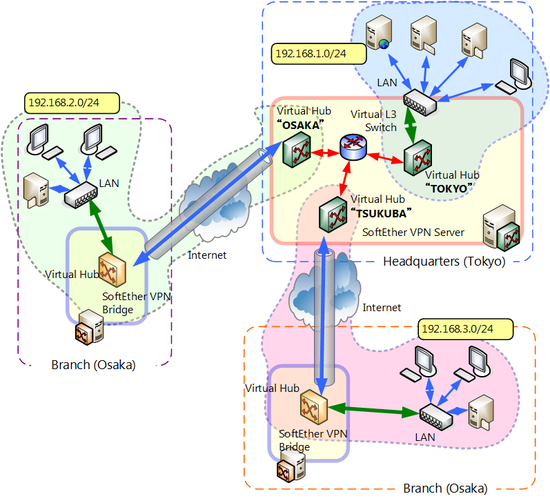
\includegraphics[scale=0.45]{img/softether_l3_lan_to_lan}
        \caption[Configurazione LAN-to-LAN con SoftEther al layer 3]{Configurazione LAN-to-LAN con SoftEther al layer 3.
          \url{https://www.softether.org/@api/deki/files/326/=10-6-1.png?size=webview}}
          \label{fig:softether_l3_lan_to_lan}
      \end{figure}
    \end{enumerate}
  \end{itemize}
\end{itemize}
SoftEther possiede alcune caratteristiche molto interessanti, oltre a quelle già citate:
\begin{description}
  \item[\textbf{VPN over ICMP} e \textbf{VPN over DNS}]Due opportunità non completamente stabili (il sito ufficiale stesso
  riporta che a volte si verificano degli errori) per il quale si incapsula il traffico in pacchetti ICMP
  o DNS per bypassare anche i firewall più stringenti. Occorre valutare \textit{quanto}
  siano stringenti tali firewall, perché anche queste soluzioni potrebbero non essere
  praticabili (ad esempio se si usa un server DNS interno e sul firewall si configura l'abilitazione
  al protocollo DNS solo se proveniente da tale server)\cite{softether-vpn-over-icmp}.
  \item[\textbf{NAT Traversal}]Se il server si trova dietro ad un NAT, è comunque possibile connettersi poiché
  esso si occupa di fare continue connessioni verso l'esterno in modo che, quando un client tenta di connettersi
  il NAT lascia passare la connessione \cite{softether-dynamic-dns-nat-trav}.
  \item[\textbf{Dyamic DNS}]Non occorre che si possieda un indirizzo IP statico per identificare il server.
  Gratuitamente SoftEther registra un nuovo nome DNS per ciascun server che viene installato, ed aggiorna
  automaticamente tale nome sulla base degli assegnamenti degli ISP (verificando quale sia l'IP
  del server che si connette all'infrastruttura SoftEther).
  \item[\textbf{SecureNAT}]Si tratta di una tecnologia sviluppata appositamente per SoftEther ed è integrata
  nel server e nel \textit{VPN Bridge}, e consiste di un DHCP+NAT eseguiti interamente in userspace\cite{softether-exploit-securenat}.
  Per ciascun \textit{Virtual Hub} è possibile abilitare questa funzione, ciò fa sì che si crei
  una nuova interfaccia di rete virtuale connessa al \textit{Virtual Hub}
  come se fosse un altro computer collegato in VPN, ed infatti, per gli altri host, la scheda virtuale appare proprio
  come un altro computer. Può essere usato per vari scopi:
  \begin{itemize}
    \item Network Gateway: \textit{SecureNAT} può essere usato come alternativa al \textit{Local Bridge} per
    connettere un \textit{Virtual Hub} alla rete fisica. Si usa una nuova interfaccia virtuale che viene connessa al \textit{Virtual Hub}.
    \item DHCP Server: è possibile scegliere di abilitare solo la funzione di DHCP Server in \textit{SecureNAT}, pertanto
    tale server assegnerà gli indirizzi IP agli alle interfacce dei client connesse al \textit{Virtual Hub} a cui
    l'interfaccia \textit{SecureNAT} è collegata.
    \item Remote Access. Questa è in assoluto la caratteristica più interessante, le cui potenzialità andrebbero studiate
    nel dettaglio. Normalmente, quando ci si vuole connettere ad una rete da remoto è
    necessario installare su in essa \textit{VPN Server}, e di conseguenza connettersi da un client. Usando \textit{SecureNAT}
    è invece possibile invertire questo paradigma. La figura \ref{fig:securenat} illustra la topologia che si realizza.\\
    \begin{figure}
      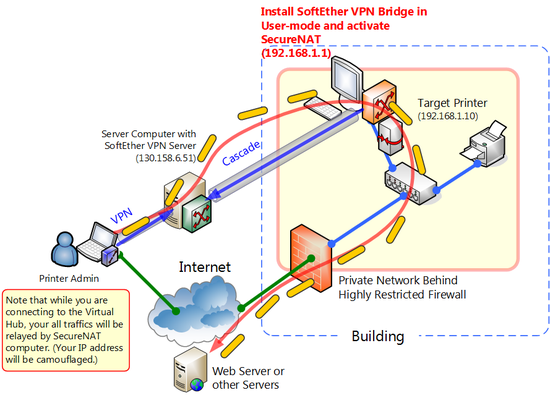
\includegraphics[scale=0.55]{img/softether_securenat}
      \caption[La topologia realizzata con \textit{SecureNAT}]{
        La topologia realizzata con \textit{SecureNAT}.
        \url{https://www.softether.org/@api/deki/files/342/=10-11-9.png?size=webview}}
        \label{fig:securenat}
    \end{figure}
    Senza scendere troppo nei dettagli, si illustrano gli step necessari. Per \textit{rete remota} si intende la rete a cui
    ci si vuole connettere, per \textit{rete principale} si intende la rete da cui la connessione parte, ovvero
    la rete da cui l'utente fisicamente si collega.
    \begin{enumerate}
      \item Sulla rete principale si crea un server con \textit{Virtual Hub}
      \item su un host della \textit{rete remota} si installa e si esegue il \textit{VPN Bridge}
      \item si abilita la funzione di \textit{SecureNAT} sul \textit{VPN Bridge}
      \item si configura il server della rete principale per creare una nuova connessione verso il \textit{VPN Bridge}.\\
      Ciò che accade è che si è stabilita una \textit{cascaded connection} tra il bridge ed il server (il \textit{Virtual Hub}
      del server).
      \item Per utilizzare davvero questo funzionalità l'utente usa un client VPN e si connette al server. La NIC
      del client sarà configurata dal DHCP Server di \textit{SecureNAT} integrato nel bridge,
      ed il bridge stesso sarà il suo default gateway. Tutto il traffico del client andrà verso il bridge, e dal bridge poi
      uscirà su internet (usando l'IP pubblico del NAT dietro a cui c'è il bridge). Grazie a ciò che SoftEther offre,
      non è necessaria alcuna configurazione nella rete remota (se non l'installazone del \textit{VPN Bridge}).
    \end{enumerate}
  \end{itemize}
  \item[\textbf{Performance}]Secondo dei test eseguiti nel 2012 SoftEther \textit{VPN Server} è più veloce (maggiore throughput) di tutte le
  altre alternative. Il grafico in figura \ref{fig:softether-performance} mostra il risultato dei test. Si tenga comunque
  conto che sono benchamrk vecchi di 6 anni, e che nel frattempo anche i concorrenti si sono evoluti.
\end{description}
\begin{figure}
  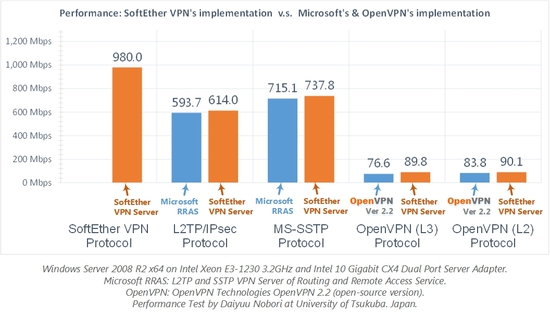
\includegraphics[scale=0.4]{img/softether_perf}
  \caption[Comparazione performance delle diverse tecnologie VPN]{
    Comparazione performance delle diverse tecnologie VPN (2012).
    \url{https://www.softether.org/@api/deki/files/12/=1.3.jpg}}
  \label{fig:softether-performance}
\end{figure}

\subsection{SoftEther e MoonCloud}
Dopo aver analizzato SoftEther ora si vedono quali sono le possibili configurazioni per un suo uso in MoonCloud.
Si è valutata come migliore soluzione quella basata su incapsulamento in HTTPS di L3, ovvero utilizzare
il protocollo SoftEther.
La prima distinzione sta nel dove posizionare il server.
\begin{description}
  \item[\textbf{Local Server}]Installare il server nella rete MoonCloud pone un problematica
  non così banale, cioè la necessità (non mandatoria ma caldamente consigliata) di
  disporre di una scheda di rete da poter configurare in modalità promiscua, ovviamente
  a livello di VM. E' possibile che dei cloud provider non consentano questo.
  Nella rete target si porterebbe un'appliance con \textit{VPN Bridge}.
  \item[\textbf{Remote Server}]In questa configurazione, se l'implementazione
  di NAT Traversal di SoftEther lo consente, sarebbe possibile per i client raggiungere
  il server nella rete target anche se dietro ad un NAT. Occorrerebbe poi valutare se utilizzare
  un unico client in MoonCloud (\textit{RSSC}) oppure diversi (\textit{RSMC}); ovviamente
  per \textit{unico client} si intende un \textit{unico} client per ciascuna rete.
\end{description}
In ogni caso, nemmeno SoftEther può eliminare la necessità di configurare rotte
nella rete target, se non con l'utilizzo del già citato \textit{NAT al contrario}.

Oltre a queste soluzioni classiche, si sarebbe potuto sfruttare anche \textit{Secure NAT}.
Si tratta di una modalità interessante, che avrebbe richiesto uno studio approfondito
per capire come potesse davvero aiutare lo use case in questione.
In questo caso:
  \begin{itemize}
    \item l'appliance è costituita dal \textit{VPN Bridge};
    \item in MoonCloud si installa il server;
    \item i container sono client VPN che si connettono al server.
  \end{itemize}


\subsection{Conclusioni}
Per SoftEther, in forza del NAT Traversal, si è consigliato di realizzare una topologia
\textit{Remote Server}, eventualmente combinabile con il Dynamic DNS fornito
da SoftEther o con uno gestito da MoonCloud.
Un ulteriore ed importante vantaggio è che SoftEther utilizza HTTPS. Per tutte queste
ragioni SoftEther è stata inizialmente preferita rispetto ad OpenVPN.

\section{IPsec}
\subsection{Overview}
IPsec è una suite di protocolli usata per rendere sicuro il livello 3 dello stack di
rete. Mediante crittografia si realizza una connessione che garantisce
numerose proprietà di sicurezza. Due protocolli disponibili:
\begin{itemize}
  \item \textit{AH - Authentication Header}: integrità ed autenticazione (no IP spoofing) del pacchetto con HMAC.
  E' fondamentale comprendere che questa soluzione non è compatibile con NAT.
  \item \textit{ESP - Encapsulating Payload}: confidenzialità del pacchetto mediante cifratura simmetrica.
  Opzionalmente in \textit{ESP} si può abilitare direttamente l'autenticazione e l'integrità,
  si consiglia questa strada.
\end{itemize}
Si può abilitare anche la protezione da replay attacks.\\

Il terzo membro della suite IPsec è \textit{IKE -- Internet Key Exchange} che viene
utilizzato per negoziare i parametri per i due protocolli precedentemente citati.

IPsec (sia \textit{AH} o \textit{ESP}) può funzionare in due modalità:
\begin{itemize}
  \item \textit{Transport Mode}: aggiunta di un nuovo header (AH o ESP) tra l'header IP
  ed il payload.
  Il suo uso tipico è quello in comunicazioni \textit{dirette} tra due host, che non si affidano a
  due gateway di confine per eseguire IPsec.
  \item \textit{Tunnel Mode}: si crea un nuovo pacchetto. Esso è costituito da
  un nuovo header IP, dall'header IPsec (AH o ESP), e quindi dal payload di IPsec, costituito dal
  vecchio header IP e dal suo payload.
\end{itemize}

Per ciò che concerne IKE, è un protocollo abbastanza complesso. Brevemente, la negoziazione
dei parametri avviene in due fasi:
\begin{itemize}
  \item nella \textit{phase 1} viene negoziata una \textit{Security Association} (set di parametri)
  bidirezionale, utilizzata nella
  \item \textit{phase 2}; in questa fase si utilizza la SA precedente per negoziare i
  parametri per la sessione IPsec, tra essi vi sono le chiavi di sessione (stabilite con
  uno scambio Diffie-Hellman).
\end{itemize}
Attualmente, è disponibile la versione 2 di IKE. Si tratta di un upgrade importante sotto molteplici punti
di vista, ed è fortemente consigliata una implementazione di IPsec che supporti IKEv2.
La porta standard utilizzata è la 500 UDP.


L2TP (Layer 2 Forwarding Protocol) è un protocollo standard il cui scopo è quello
di realizzare una connessione punto-punto, per cui non include vere funzionalità
di sicurezza. L'RFC 3193 standardizza l'uso combinato di IPsec per creare una
connessione sicura, sulla quale si negoziano
i parametri L2TP \cite{RFC3193}.


Per realizzare VPN con IPsec tipicamente si utilizzano due configurazioni:
\begin{itemize}
  \item L2TP on IPsec (negoziazione di L2TP su un canale IPsec sicuro--\textit{ESP Transport Mode}
  \item IPsec with IKEv2.
\end{itemize}


Lo stack tipico di IPsec su Linux è il seguente:
\begin{itemize}
  \item ESP ed AH implementati nel kernel, per cui molto veloci
  \item demone IKE in \textit{userspace}, negozia le policy per la sessione e le
  passa al kernel.
\end{itemize}
L'implementazione IKE di riferimento per Linux, sebbene sia disponibile anche
cross-platform, è \texttt{strongSwan} \cite{strongswan}. Maggiori dettagli su essa sono descritti
tra qualche riga.


E' possibile realizzare configurazioni Remote Access e LAN-to-LAN. IPsec è uno stack
complesso, e configurarlo nella maniera corretta non è facile, tuttavia non è nemmeno
impossibile, il sito di strongSwan è ricco di esempi e di documentazione \cite{strongswan-example}.
Nella terminologia IPsec con strongSwan si definiscono i seguenti termini:
\begin{itemize}
  \item \textit{roadwarrior} è il client, cioè il dispositivo che si connette da remoto alla rete (\textit{initiator})
  \item \textit{VPN Gateway} è il server che accetta le connessioni (\textit{responder}).
\end{itemize}

Da subito ci si è concentrati su un setup basato su IKEv2, poiché si tratta della
versione più recente del protocollo. Non si è considerato IPsec con L2TP
visto che utilizza tipicamente IKEv1, ed è considerato \textit{legacy} \cite{nordvpn}.

Utilizzando strongSwan sono possibili moltissime forme di autenticazione, distinguendo tra:
\begin{itemize}
  \item autenticazione degli host, può essere fatta con PSK (fortemente sconsigliato) o certificati X509
  \item autenticazione degli utenti, in questo caso è possibile usare anche un
  server RADIUS.
\end{itemize}
Si tenga presente che l'autenticazione degli utenti è fatta \textit{on top} dell'autenticazione
degli host.
Per ciò che concerne un'autenticazione basata su certificati, occorre seguite gli stessi
fatti già descritti per OpenVPN, ovvero creare chiavi/certificato per la CA, quindi generare
certificati con essa, ecc\ldots


Come per la maggior parte dei software Linux, la configurazione di strongSwan viene
fatta mediante file di configurazione.
E' di particolare rilevanza configurare correttamente \textit{quali} indirizzi IP vengono
incapsulati nel tunnel IPsec, perché le policy presenti nel kernel descrivono anche questo,
e se un pacchetto ha sorgente o destinazione IP non corretti sarà droppato dal kernel.

strongSwan è una soluzione molto interessante e completa, alcune caratteristiche
che meritano una menzione sono relative ad alcuni algoritmi crittografici supportati:
\begin{itemize}
  \item supporto a certificati \texttt{Ed25519} (istanza dell'algoritmo di firma digitale
  \textit{EdDSA} basato su \textit{Twisted Edward Curves},
  particolarmente interessante per numerosi motivi tra cui le
  performance e la facilità di implementazione)
  \item supporto ad alcuni algoritmi a chiave pubblica post-quantistici (basati su
  problemi matematici per i quali i computer quantistici non portano alcun vantaggio
  nella loro soluzione) come \texttt{NTRU} (\textit{lattice-based cryptography}).
\end{itemize}
strongSwan offre NAT Traversal basato su UDP.


\subsection{IPsec e MoonCloud}
In IPsec, una volta
che le policy sono state stabilite, non vi è davvero distinzione tra chi sia client e server.
Si distingue solamente nelle topologie che si realizzano, ed in base a dove si posiziona il client cioè
l'\textit{initiator}.
Sono quindi possibili sia configurazioni \textit{RS} ed \textit{LS}, un server nella rete target
potrebbe sfruttare il NAT Traversal che strongSwan offre, occorrerebbe valutarne l'efficacia.
La topologia \textit{LS} è sempre possibile.


\subsection{Conclusioni}
Si è consigliata una topologia \textit{RS}, posto che il NAT Traversal consente
la raggiungibilità dall'esterno, in caso contrario \textit{LS}.
Vi sono diverse voci fondate dalle dichiarazioni di Snowden, secondo cui l'\textit{NSA avrebbe volontariamente
indebolito il protocollo}\ldots\footnote{La bibliografia in questo è il corso di Sicurezza delle Reti.}
Altre voci invece riportano di come l'NSA sia in grado di rompere sessioni IPsec
configurate con PSK (\cite{ipsec-nsa}).
Si rilevano infine due problemi principali:
\begin{itemize}
  \item complessità: IPsec è costituito da numerosi protocolli e non è generalmente considerato
  facile da configurare, in particolar modo occorre prestare attenzione alle policy che specificano
  quali indirizzi IP possono essere incapsulati
  \item supporto ad UDP: è indispensabile che il traffico UDP sia abilitato perché IKE funziona
  su tale protocollo.
\end{itemize}


\section{Altre tecnologie}
\subsection{SSTP}
\textit{Secure Socket Tunneling Protocol} è il protocollo VPN di nuova generazione sviluppato
da Microsoft \cite{sstp}, il cui client è nativamente integrato in Windows. Il server è tipicamente
disponibile nelle versioni Server di Windows, tuttavia esistono dei cloni gratuiti, come
SoftEther; vi sono anche client per Linux.\\
SSTP incapsula in TLS , quindi un protocollo
sicuro, tuttavia non offre particolari vantaggi rispetto a SoftEther, inoltre il supporto
per piattaforme non-Microsoft va verificato.

\subsection{OpenConnect}
\textit{DTLS - Datagram Transport Layer Security} è uno standard RFC che specifica
una sorta di di TLS su UDP, per fornire le stesse garanzie di sicurezza che TLS dà
su TCP \cite{RFC6347}. Come tale, può essere utilizzato per costruire VPN.\\
\texttt{Cisco Any Connect} è una soluzione VPN basata su DTLS e HTTPS, e
\texttt{OpenConnect} è una soluzione open source sia client sia server compatibile
\cite{cisco-vpn} \cite{openconnect-client} \cite{openconnect-server}.
OpenConnect fornisce una configurazione simile ad OpenVPN \cite{openconnect-server-conf}.
Per ciò che concerne il funzionamento, vi è una prima fase di
autenticazione su HTTPS, il traffico poi procede su DTLS, eventualmente si sposta su
HTTPS se UDP non è supportato. Da questo punto di vista non avevo rilevato particolari
vantaggi rispetto a SoftEther o OpenVPN.


\subsection{OpenSSH}
\textit{Secure SHell} è un protocollo usato da lungo tempo per creare sessioni di login remoto.
La prima versione del protocollo SSH mirava semplicemente a rendere sicura una
sessione telnet, mentre la versione 2 rende disponibile un protocollo di trasporto
sicuro sul quale è possibile poi offrire diversi servizi multiplexati su quest'unico
protocollo.

Sono offerte vari tipi di autenticazione, tra cui username e password, oppure basata
su chiavi pubbliche (negoziate a priori).

Uno dei software più diffusi che implementano questo protocollo è OpenSSH.

Le ultime versioni di tale software consentono anche di creare
diversi tipi di tunnel altre al classico di login remoto, tra cui anche tunnel verso
host remoti al livello 2 o 3. Si tratta a tutti gli effetti di una VPN, poiché
offre una connettività completa al livello desiderato (non si tratta di
\textit{SSH reverse tunnel} o \textit{forwarding})
\cite{ssh-vpn-ubuntu} \cite{ssh-vpn-debian}.

Per funzionare si utilizzano delle interfacce di rete virtuali
su client e sul server. Si è tratta di una soluzione interessante, basata su un
protocollo ben noto, tuttavia, ad una prima analisi, non si sono rilevati
particolari vantaggi rispetto a SoftEther od OpenVPN.

\subsection{WireGuard}
\textit{WireGuard}\cite{DBLP:conf/ndss/Donenfield17} è una moderna soluzione VPN per Linux, creata con i seguenti obiettivi:
\begin{itemize}
	\item facile da configurare
	\item sicurezza mediante crittografia:
	      \begin{itemize}
	      	\item autenticazione con chiavi pubbliche Diffie-Hellman su curva ellittica \textit{X25519}
	      	      e scambiate a priori
	      	\item pacchetti scambiati usando \textit{ChaCha20-Poly1305} con \textit{Authenticated
	      		Encryption with Associated Data}
	      		\item chiavi di sessione rinegoziate periodicamente
	      	\end{itemize}
	      	\item elevate performance
	      	\item minimalità: key exchanging, aggiunta e rimozione delle rotte dal kernel
	      	      non sono intenzionalmente gestite.
	      \end{itemize}
	      WireGuard è implementato come un modulo del kernel Linux e come tale riesce ad essere
	      molto performante, i benchamrk forniti dagli autori riportano un throughput vicino
	      ad 1 Gbps figura \ref{fig:wireguard-performance}).
	      Lavora a livello 3 ed i partecipanti sono dei peer,
	      il protocollo di trasporto è UDP. Per funzionare correttamente con il NAT vi è
	      la possibilità di configurare i peer per mandarsi periodicamente dei keep-alive.
	      
	      
	      Poiché è una proposta molto interessante, è stata analizzata pià in dettaglio rispetto
	      alle altre proposte di questa sezione. Per configurare un peer,
	      posto di avere la chiave pubblica dell'altro endpoint, occorre:
	      \begin{itemize}
	      	\item aggiungere una una nuova interfaccia virtuale e configurarla specificandone
	      	      l'indirizzo IP, sarà l'indirizzo IP del tunnel VPN
	      	\item aggiungere le rotte verso le reti indirizzate dagli altri endpoint alla scheda
	      	      di rete virtuale
	      	\item Configurazione della \textit{cryptokey routing table}, ovvero specificare
	      	      quali remote sono responsabili di quali reti a livello di VPN\cite{wireguard-quick-start}.
	      \end{itemize}
	      \begin{figure}
	      	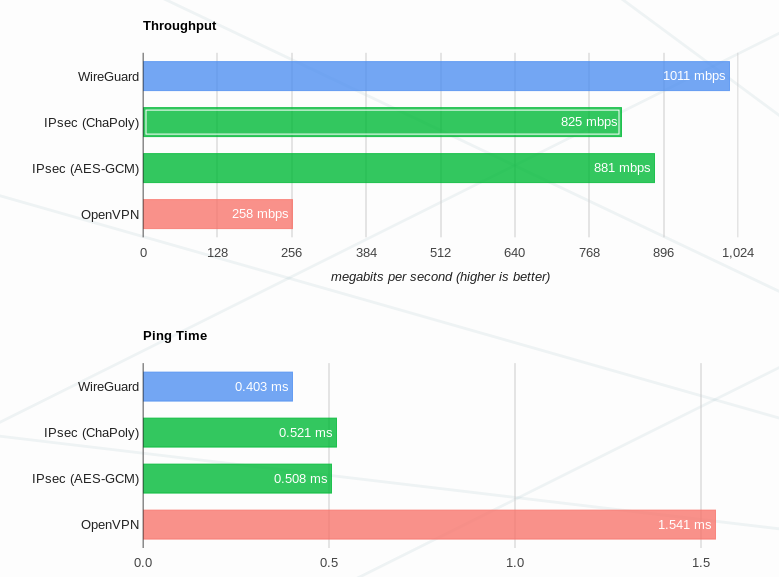
\includegraphics[scale=0.45]{img/wireguard_performance}
			  \caption[Benchmark tra IPsec, OpenVPN e WireGuard]{Benchmark tra IPsec, OpenVPN e WireGuard.
			  	OpenVPN è la soluzione più lenta poiché è l'unica implementata nello user-space.
	      		\url{https://www.wireguard.com/performance/}}
	      	\label{fig:wireguard-performance}
		  \end{figure}
		  Un interfaccia WireGuard può gestire più peer, ed occorre che le chiavi pubbliche di tutti
	      i peer a cui ci si vuole connettere siano presenti su tutti i partecipanti.
		  WireGuard ha un grande potenziale, tuttavia è poco configurabile. Questo ha il vantaggio
		  di rendere tale soluzione molto facile da configurare, al prezzo di, semplicemente, avere
		  molte meno opzioni su cui intervenire. In fase di scelta
	      finale, questa soluzione è stata infine scartata perché funzionante su UDP.
	      
	      
	      
	      \subsection{IPsec/L2TPv3 e EtherIP/IPsec}
	      \begin{itemize}
	      	\item L2TP versione 3 è l'ultimo aggiornamento del protocollo L2TP, principalmente implementato in
	      	      device Cisco. Analogamento ad L2TP, è possibile usarlo per creare VPN LAN-to-LAN al livello 2.\\
	      	      Viene supportato dai principali produttori di apparati di rete, oltre che da Linux.
	      	\item EtherIP è un protocollo per l'incapsulamento di frame Ethernet in frame IP, il cui scopo è quello
	      	      di connettere tra loro diverse LAN a livello 2.
	      \end{itemize}
	      Entrambi i due protocolli devono essere incapsulati in IPsec per ottenere una VPN che garantisca proprietà
	      di sicurezza.
	      EtherIP è
	      supportato da Linux ed in SoftEther VPN Server.\\
	      Le due tecnologie sono in qualche modo simili, poiché realizzano connessioni a livello 2. Nel caso in cui
	      MoonCloud abbia esigenze di lavorare al livello 2, queste soluzioni sono da prendere in considerazione, sebbene
	      anche OpenVPN e SoftEther supportino VPN a questo layer.
	      
	      
	      \subsection{PPTP}
	      Il protocollo \textit{PPTP - Point To Point Tunneling Protocol} è un protocollo
	      \textit{legacy}, sviluppato da Microsoft e non più sicuro, sebbene (purtroppo)
	      ancora usato.
	      Questo protocollo offre VPN, ma non è assolutamente una soluzione praticabile per
	      MoonCloud.

\section{Conclusioni}
In conclusione del capitolo si fornisce un riassunto di pro e contro delle principali
tecnologie.
Nonostante WireGuard non sia stato analizzato
in dettaglio, viene comunque inserito in questa lista grazie ai suoi vantaggi.
\begin{description}
  \item[\textbf{OpenVPN}]
  \begin{itemize}
    \item ampio supporto e documentazione
    \item sicurezza basata su TLS e protocollo custom assimilabile ad esso
    \item vari tipi di autenticazione
    \item possibile connessione anche al layer 2
    \item topologie consigliate:
    \begin{enumerate}
      \item \textit{LS} con client in \textit{NAT al contrario}
    \end{enumerate}
    \item Contro:
    \begin{itemize}
      \item utilizzo di TLS su protocollo custom, quindi il traffico non riesce
      ad essere \textit{spacciato} completamente per HTTPS
      \item necessaria gestione dei certificati
    \end{itemize}
  \end{itemize}
    \item[\textbf{SoftEther}]
    \begin{itemize}
      \item multi-protocol e multi-platform
      \item incapsulamento in HTTPS
      \item possibile connessione anche al layer 2;
      \begin{itemize}
        \item bypassa la maggior parte dei firewall
      \end{itemize}
      \item NAT Traversal del server
      \item Dynamic DNS
      \item VPN over ICMP e over DNS
      \item topologia consigliate:
      \begin{enumerate}
        \item \textit{RS} senza bisogno di abilitare port forwarding sfruttando
        NAT Traversal
        \item \textit{LS}
      \end{enumerate}
      \item Contro:
      \begin{itemize}
        \item necessità di una seconda NIC sul server in modalità promiscua
        \item documentazione buona per Windows, meno per Linux
      \end{itemize}
    \end{itemize}
    \item[\textbf{IPsec}]
    \begin{itemize}
      \item IKEv2 dà ampia scelta di configurazioni
      \item sicurezza mediante ESP (cifratura payload pacchetto IP)
      \item NAT Traversal
      \item topologie consigliate:
      \begin{enumerate}
        \item \textit{LS}
        \item \textit{RS}
      \end{enumerate}
      \item Contro:
      \begin{itemize}
        \item setup non facile
        \item necessaria gestione dei certificati
        \item non passa tutti i firewall poiché si tratta di un nuovo protocollo
        che deve essere abiltato
        \item voci di indebolimento da parte dell'NSA
      \end{itemize}
    \end{itemize}
    \item[\textbf{WireGuard}]
    \begin{itemize}
      \item molto più performante di ogni altra soluzione
      \item altamente sicuro
      \item keep-alive per funzionare con NAT
      \item Contro:
      \begin{itemize}
        \item il sito stesso non lo definisce \textit{production ready};
        \item necessità di scambiare chiavi a priori
        \item traffico UDP potrebbe essere bloccato
      \end{itemize}
    \end{itemize}
\end{description}
La soluzione SoftEther con HTTPS è sembrata essere quasi perfetta, se il NAT Traversal
funzionasse come dichiarato si sarebbe potuta creare una topologia \textit{RS}.
Per firewall molto stringenti sono sembrate molto interessanti le possibilità di incapsulamento
in ICMP  e DNS, sebbene dichiarate come non completamente affidabili.

L'opzione IPsec con IKEv2 è altrettanto valida, il principale svantaggio è che i firewall più stringenti
potrebbero bloccare il traffico \textit{ESP}. In tal caso si può incapsulare \textit{ESP} in \textit{UDP},
ma comunque si richiede che il traffico UDP sia permesso (porta 500).

Come prima soluzione si è scelta SoftEther, ma infine quella utilizzata è OpenVPN. Il
prossimo capitolo ne affronta la configurazione nel dettaglio.

